\addsec{Vorlesung 12 - Lösungen}

\minisec{Übungsaufgabe 1:}
\begin{itemize}
    \item Der NRZ-Code übersetzt die Nutzdaten einfach in 2 Signalpegel (z. B. 0 → Pegel 0, 1 → Pegel 1).
    \item Der NRZ-I-Code übersetzt eine 1 in den Nutzdaten in einen Zustandswechsel im Signalpegel, also
    0 → kein Pegelwechsel im Signal, 1 → Pegelwechsel im Signal
    \item Der Manchester-Code (IEEE 802.3) übersetzt eine 0 in einen Pegelwechsel von +U nach -U, und
    eine 1 in einen Pegelwechsel von -U nach +U (jeweils gleich lange).
\end{itemize}

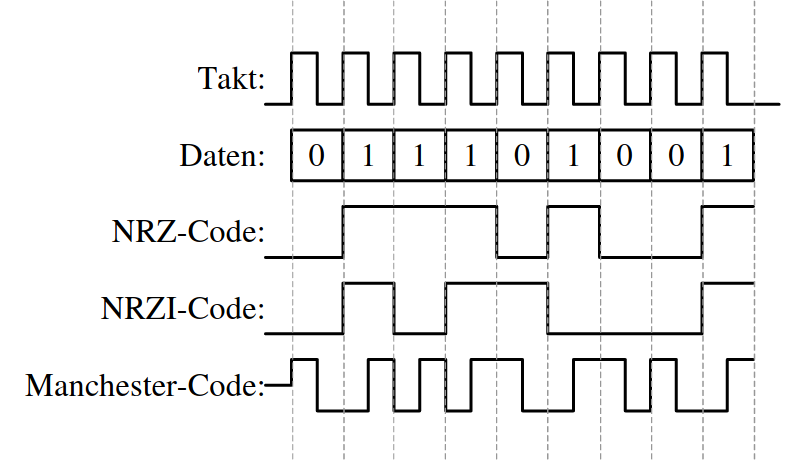
\includegraphics[width=\textwidth]{img/vorlesung12_uebungsaufgabe1_loesung}
